\section{Proposed Methodology}
\subsection{Architecture and the Shared Representation}
Fig.~\ref{fig:architecture} shows the application components and their principal relationships. A Next.js workspace exposes the resource canvas, configuration forms, saved sketches, resource observations, and conversation interface. Express owns protected application APIs, persistence coordination, and AWS operations. FastAPI hosts the LangGraph workflow, while PostgreSQL stores the application's durable records. The shared TypeScript graph contract is imported by the client and server; it is not an HTTP service and is not directly imported by Python. Separating it from either interface allows returned AI drafts and user-imported graph descriptions to meet the same application acceptance boundary~\cite{cloudcanvas}.
\begin{figure}[t]
\centering
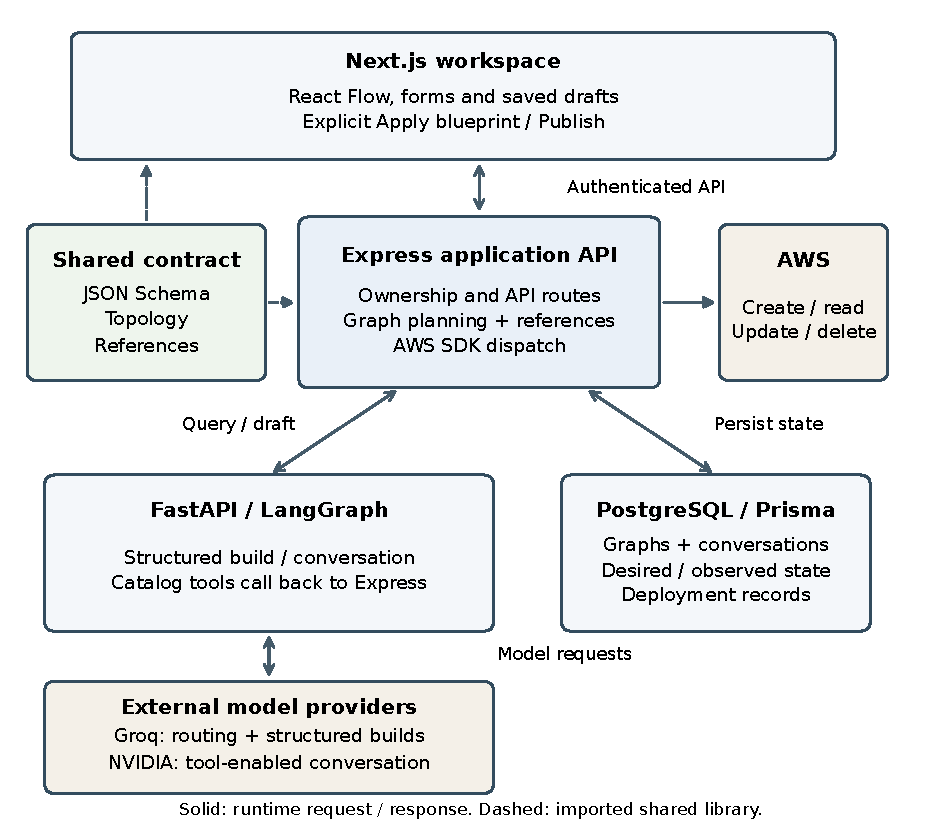
\includegraphics[width=.98\linewidth]{architecture.pdf}
\caption{CloudCanvas architecture. Solid connections denote runtime communication; dashed connections denote use of the shared TypeScript library. AI returns advice or drafts, while application code controls AWS mutation.}
\label{fig:architecture}
\end{figure}
The contract declares supported service types, configuration schemas, edge compatibility, graph diagnostics, and reference rules. Python uses separate Pydantic definitions for structured responses, so the server validates returned builds again rather than assuming language-level equivalence. This duplicates some type knowledge but creates an explicit runtime trust boundary. JSON Schema provides an inspectable document definition, and Ajv is configured with defaults, all-error reporting, and non-strict schema compilation~\cite{jsonschema2022,ajv}. Those choices support normalization and useful diagnostics. They do not turn optional draft fields into deployment-ready configuration.

\subsection{Layered Graph Validation}
Algorithm~\ref{alg:validation} describes the logical validation sequence. Schema checking first rejects unsupported document shapes and values. The topology stage then checks unique node identifiers, known edge endpoints, self-edges, compatible attachments, duplicate edges, and the single-origin constraint for CloudFront. It derives predecessor sets and a topological order. Reference validation recursively traverses configuration values, accepting reference strings only when their syntax is exact and their source is a direct predecessor. This explicit association prevents an apparently meaningful reference from bypassing the graph's dependency representation.
\begin{algorithm}[t]
\caption{Validate a proposed CloudCanvas graph}
\label{alg:validation}
\KwIn{Candidate graph $G$; shared schema; permitted type relation set}
\KwOut{Normalized graph and topological order, or diagnostics}
Check $S(G)$; return diagnostics if schema validation fails\;
Require unique identifiers for every node in $V$\;
Initialize predecessor sets and in-degree counters\;
\ForEach{edge $(u,v)\in E$}{
Require known distinct endpoints and a permitted type pairing\;
Reject duplicate edges and multiple CloudFront origins\;
Record the predecessor and increment the target in-degree\;
}
Compute a topological order; reject if it does not cover $V$\;
\ForEach{configuration value containing reference syntax}{
Require the exact reference form and extract $(u,k)$\;
Require $u\in\operatorname{Pred}_{G}(v)$ for its consuming node $v$\;
}
\Return{accepted normalized graph and order}\;
\end{algorithm}
For an accepted dependency edge, the order $\pi$ must satisfy
\begin{equation}
 (u,v)\in E\ \Longrightarrow\ \pi(u)<\pi(v).
 \label{eq:order}
\end{equation}
The notation $\pi(v)$ denotes a node's position in the execution ordering. The supported type-pair relation is itself acyclic, so the tested cyclic fixture also violates compatibility; the experiment does not isolate the cycle-detection branch. Although the planner follows a Kahn-style structure, its current per-edge node searches and array-based queue can introduce $O(|V||E|+|V|^2+B)$ work, where $B$ denotes configuration traversal size. We consequently avoid a general linear-time or large-graph scalability claim.

\subsection{Reviewed AI Drafting and Workspace Persistence}
The active LangGraph workflow routes AWS construction requests to a structured Groq branch and general conversation to a NVIDIA branch with tool calls~\cite{langgraph}. Tools supply resource-support guidance, web search, and an authenticated callback for AWS catalog choices. The conversation controller includes bounded catalog context and prior conversation text, but does not automatically serialize the complete current canvas into the model prompt. Provider clients are instantiated lazily; a defined alternative Llama wrapper is not part of the active graph. Model outputs are text advice or draft graphs, not unrestricted cloud mutation commands.

Fig.~\ref{fig:workflow} illustrates the user-facing path from proposal to observed outcome. Applying a blueprint and publishing infrastructure are separate decisions. Accepted blueprint replacement runs transactionally, remaps persisted node identifiers and configuration references, and is blocked while associated resources remain non-terminated. Manual canvas changes use incremental APIs and queued debounce persistence; undo and redo operate on editor snapshots. The separation makes drafts inspectable, but a full replacement is not a verified incremental editing engine. The paper evaluates validation before these application decisions. The effectiveness of user review would require a separate study.
\begin{figure}[t]
\centering
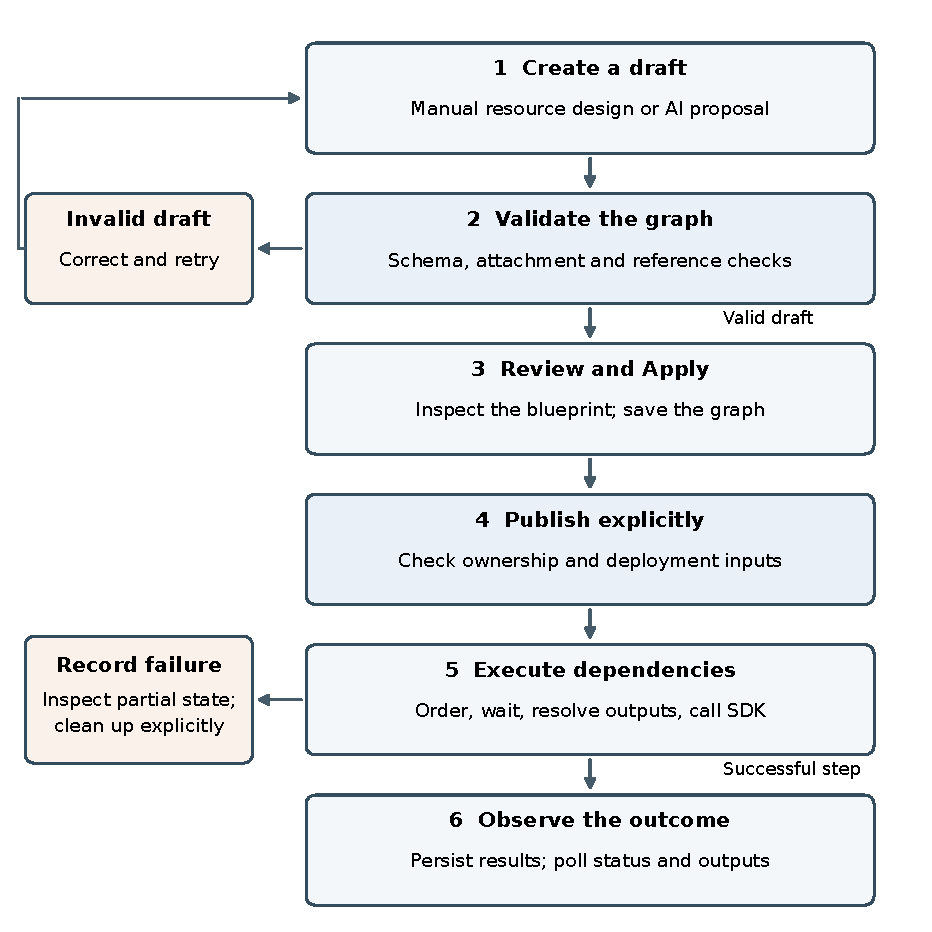
\includegraphics[width=.96\linewidth]{workflow.pdf}
\caption{Reviewed workflow, including rejection before application and explicit handling of partial execution failure. Publish performs additional checks beyond draft acceptance.}
\label{fig:workflow}
\end{figure}

\subsection{Execution, Observation, and Cleanup}
Publishing checks the owned sketch and connection, validates supported deployment inputs, decrypts the connection credentials, and constructs the execution order. For each node, the controller waits for direct dependencies, resolves configuration references against stored or refreshed outputs, and dispatches the appropriate AWS SDK operation~\cite{awssdk}. Unlike draft reference validation, resolution checks the requested output field's availability. Resource records distinguish desired configuration, observed state, external identifiers, management ownership, and errors. Deployment records preserve requests, outcomes, and timestamps. This accounting makes partial progress visible but is not a transaction spanning AWS and PostgreSQL.

Most successful create returns initially become application-level running records; CloudFront remains provisioning until later observation. The editor triggers status refresh periodically, and dependent operations explicitly wait for required readiness. Therefore, an accepted API response, the application's running label, and workload health remain different observations. A user can inspect outputs or request cleanup. Bulk cleanup reverses dependency order and stops at a pending or failed result; adopted resources are detached locally while managed resources are deleted. S3 content/version deletion and forced ECR deletion are consequential operations, and asynchronous CloudFront cleanup depends on subsequent refresh calls.

This prototype intentionally retains important operational limitations. Execution runs within an Express request without a durable worker, atomic per-sketch reservation, automatic rollback, or general idempotency guarantee. Some error paths can leave pending deployment receipts. Normal node configuration updates are blocked for live resources even though update dispatchers exist. Express protects sketch and connection APIs with JWT ownership checks, but the present Google profile exchange and FastAPI service boundary require further hardening. These limitations are part of the described implementation, not capabilities supplied implicitly by the libraries. Docker Compose packages the client, server, AI service, and database with internal networking and migration startup~\cite{compose}; packaging alone does not address these lifecycle and security gaps.
